\documentclass[border=4pt]{standalone}

\usepackage[T1]{fontenc}
\usepackage[utf8]{inputenc}
\usepackage{amsmath}
\usepackage{xcolor}
\usepackage{tikz}
\usetikzlibrary{arrows.meta}

\begin{document}

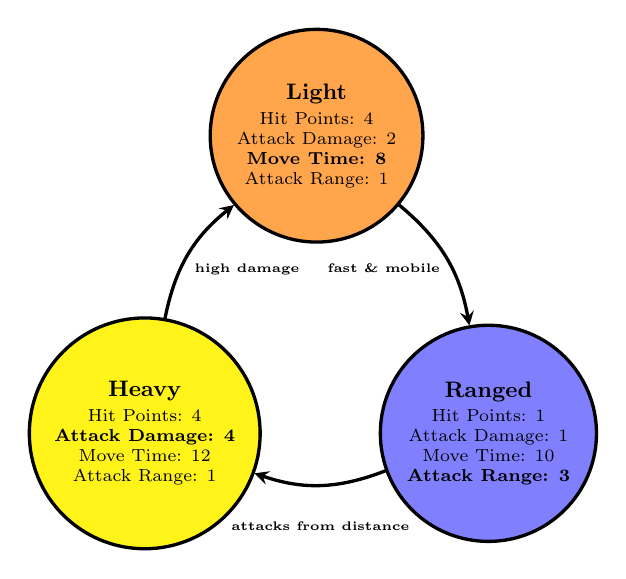
\begin{tikzpicture}[
    scale=0.9,
    every node/.style={transform shape},
    unit/.style={
        circle,
        draw,
        very thick,
        minimum size=2.5cm,
        align=center,
        font=\scriptsize
    },
    arrow/.style={
        -stealth,
        very thick,
        black,
        bend left=20
    },
    label/.style={
        font=\tiny,
        fill=white,
        inner sep=2pt,
        text=black
    }
]
    \node[unit, fill=orange!70] (light) at (90:2.8) {
        \textbf{\small Light}\\[2pt]
        Hit Points: 4\\
        Attack Damage: 2\\
        \textbf{Move Time: 8}\\
        Attack Range: 1
    };
    \node[unit, fill=yellow!90] (heavy) at (210:2.8) {
        \textbf{\small Heavy}\\[2pt]
        Hit Points: 4\\
        \textbf{Attack Damage: 4}\\
        Move Time: 12\\
        Attack Range: 1
    };
    \node[unit, fill=blue!50] (ranged) at (330:2.8) {
        \textbf{\small Ranged}\\[2pt]
        Hit Points: 1\\
        Attack Damage: 1\\
        Move Time: 10\\
        \textbf{Attack Range: 3}
    };
    \draw[arrow] (light) to node[label, midway, left, yshift=-4pt] {\textbf{fast \& mobile}} (ranged);
    \draw[arrow] (ranged) to node[label, midway, below, yshift=-12pt, font=\fontsize{4pt}{5pt}\selectfont] {\textbf{attacks from distance}} (heavy);
    \draw[arrow] (heavy) to node[label, midway, right, yshift=-6pt] {\textbf{high damage}} (light);
\end{tikzpicture}

\end{document}
